\subsubsection*{AML}

\paragraph{Overview}

AML is a memory management library designed to ease the use of complex
memory topologies and complex data layout optimizations for
HPC applications.

AML is a framework providing locality-preserving abstractions to
application developers.  In particular, AML aims to expose flexible
interfaces to describe and reason about how applications deal with data
layout, tiling of data, placement of data across hardware topologies, and
affinity between work and data.

\paragraph{Key Challenges}

Between non-uniform memory access (NUMA) to regular DRAM, the 3-D stacked
high-bandwidth memory, and the memory local to the accelerator devices such
as GPUs, the increasing depth of the memory hierarchy presents exascale
applications with a critical challenge of how to use the available
heterogeneous memory resources effectively.

Standardized interfaces to manage complex memory hierarchies are lacking,
and vendors are reluctant to innovate in this space in the absence of clear
directions from the community.  Coming up with an interface that is
sufficiently expressive to cover the emerging and projected hardware
advances, yet is simple enough and practical to be both acceptable and
useful to the applications is the key challenge that we are working on
addressing.

\paragraph{Solution Strategy}

AML provides explicit, application-aware memory management for deep memory
systems.  It offers a collection of building blocks that
are \emph{generic}, \emph{customizable}, and \emph{composable}.
Applications can specialize the implementation of each offered abstraction
and can mix and match the components as needed.  AML can be used to create,
for example, a software-managed scratchpad for multilevel DRAM hierarchy
such as HBM and DDR.  Such a scratchpad provides applications with a memory
region with a predictable high performance for critical data structures.

We provide applications and runtimes with a descriptive API for data
access, where all data placement decisions are explicit, and so is the
movement of data between different memory types.  At the same time, the API
does abstract the memory topology and other device complexities.  We focus
on optimizing data locality for current and future hardware generations;
applications provide insights for static allocations, and we can also
dynamically and asynchronously move or transform data to optimize for a particular 
device or to best take advantage of the memory hierarchy.

\begin{wrapfigure}[6]{r}{.18\textwidth}
%\vspace{-12pt}%
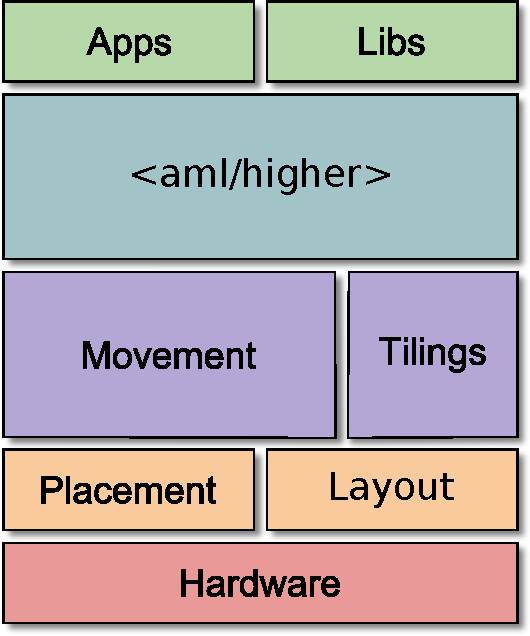
\includegraphics[width=.18\textwidth]{projects/2.3.1-PMR/2.3.1.19-Argo-PowerSteering/aml-components}
\end{wrapfigure}
AML components are built on top of hardware drivers and system
libraries (libnuma, hwloc, accelerator libraries, other ECP products).
The figure on the right depicts the major components of AML, including:
\begin{itemize}
\item Memory \emph{areas}, the location where data lives,
\item Applications data \emph{layouts} description,
\item \emph{DMA} engines, to move data across areas and layouts,
\item \emph{Tiling} schemes, the meta-structures on top of data layouts,
\item High level abstractions and helpers (\emph{replicaset}).
\end{itemize}

\paragraph{Recent Progress}

This year AML contributions are distributed across new features,
infrastructure improvements, and a new collaboration project.

As part of our effort to improve application locality, we merged
features on top of the \emph{hwloc backend}. The hwloc library exposes the machine
topology and its objects attributes. As a result, AML is able
to process the relationship between processing units and memories in
terms of latency, bandwidth, and hop distance. Additionally, AML is
able to make use of user-provided distances. Hence, it becomes
possible to enhance available performance data with benchmarked metrics.
From AML user's perspective, a new \emph{area} base block implementation
is available. It implements the \emph{preferred} allocation policy on all
memories. These memories are ordered according to a performance
criterion (e.g., bandwidth). Therefore, data can be allocated as long as
some memory is available. On top of that, data will be mapped onto the best
available memories according to a performance criterion. Furthermore,
we updated and merged the \emph{replicaset} high level abstraction which
is now available to users. In a nutshell, this abstraction will
create an area per NUMA cluster on the fastest memory of the cluster.
Then, the user can use the replicaset primitives to map data replicas
and update the latter in these areas. We previously demonstrated the use of
this facility to improve the performance of the
\emph{XSBench} application (published this year). We are working with
ExaSMR developers to offer it as an optional feature in the latest version
of the benchmark. 

Finally, the last new capability we introduced in the library is a submodule
library called \emph{excit}. Excit implements general-purpose iterators, and we
are using it to provide extensive iteration interfaces to the core building blocks
of AML, as well as custom topology object iterators. For example, we want to be
able to iterate memories of a certain type or with specific performance
abilities.

As part of our infrastructure improvements, we purchased a new machine
with heterogeneous hardware that we are using in our CI pipeline
to test new vendor backends. We are also taking advantage of the ECP CI
infrastructure as part of our development process. The development of the
library is validated by our own CI before being merged into a staging
branch. The latter is then mirrored to ECP facilities to be further tested by
an ECP CI pipeline, before being merged into our master branch. The goal is to
ensure that our master branch can always be stable on production systems. Our
ECP CI pipeline runs on Theta at ALCF and we are in the process of setting it
up at OLCF.

\paragraph{Next Steps}

We are looking to build on top of our success with XSBench and use it as a
showcase of some of the AML capabilities. Our next goal is to provide a feature
inspired by OpenMP 5 \emph{custom mappers}. An OpenMP mapper makes it possible to
describe which parts of a structure should be mapped onto
accelerator devices. As it is a recent addition to the standard, to the best
of our knowledge no compiler implements it yet. Furthermore, this feature is
limited in its ability to filter or reorganize memory during the mapping
process. We are using our \emph{tiling} abstraction to build a more
flexible interface for such a feature, based on the needs of the OpenMC
application. It will be combined with our \emph{DMA} abstraction to manage
memory transfers and might be also provided through a more straightforward
higher-level API.

Finally, we are aiming at a broad compatibility of the library with accelerator
devices.  Therefore, we are about to implement the base library abstractions on
top of the \emph{OpenCL} backend.
